\documentclass[journal,12pt,twocolumn]{IEEEtran}
%
\usepackage{setspace}
\usepackage{gensymb}
%\doublespacing
\singlespacing

%\usepackage{graphicx}
%\usepackage{amssymb}
%\usepackage{relsize}
\usepackage[cmex10]{amsmath}
%\usepackage{amsthm}
%\interdisplaylinepenalty=2500
%\savesymbol{iint}
%\usepackage{txfonts}
%\restoresymbol{TXF}{iint}
%\usepackage{wasysym}
\usepackage{amsthm}
%\usepackage{iithtlc}
\usepackage{mathrsfs}
\usepackage{txfonts}
\usepackage{stfloats}
\usepackage{bm}
\usepackage{cite}
\usepackage{cases}
\usepackage{subfig}
%\graphicspath{\figure}
%\usepackage{xtab}
\usepackage{longtable}
\usepackage{multirow}
%\usepackage{algorithm}
%\usepackage{algpseudocode}
\usepackage{enumitem}
\usepackage{mathtools}
\usepackage{tikz}
\usepackage{circuitikz}
\usepackage{verbatim}
%\usepackage{tfrupee}
\usepackage[breaklinks=true]{hyperref}
%\usepackage{stmaryrd}
\usepackage{tkz-euclide} % loads  TikZ and tkz-base
%\usetkzobj{all}
\usepackage{listings}
    \usepackage{color}                                            %%
    \usepackage{array}                                            %%
    \usepackage{longtable}                                        %%
    \usepackage{calc}                                             %%
    \usepackage{multirow}                                         %%
    \usepackage{hhline}                                           %%
    \usepackage{ifthen}                                           %%
  %optionally (for landscape tables embedded in another document): %%
    \usepackage{lscape}     
\usepackage{multicol}
\usepackage{chngcntr}
%\usepackage{enumerate}

%\usepackage{wasysym}
%\newcounter{MYtempeqncnt}
\DeclareMathOperator*{\Res}{Res}
%\renewcommand{\baselinestretch}{2}
\renewcommand\thesection{\arabic{section}}
\renewcommand\thesubsection{\thesection.\arabic{subsection}}
\renewcommand\thesubsubsection{\thesubsection.\arabic{subsubsection}}

\renewcommand\thesectiondis{\arabic{section}}
\renewcommand\thesubsectiondis{\thesectiondis.\arabic{subsection}}
\renewcommand\thesubsubsectiondis{\thesubsectiondis.\arabic{subsubsection}}

% correct bad hyphenation here
\hyphenation{op-tical net-works semi-conduc-tor}
\def\inputGnumericTable{}                                 %%

\lstset{
%language=C,
frame=single, 
breaklines=true,
columns=fullflexible
}
%\lstset{
%language=tex,
%frame=single, 
%breaklines=true
%}

\begin{document}
\newtheorem{theorem}{Theorem}[section]
\newtheorem{problem}{Problem}
\newtheorem{proposition}{Proposition}[section]
\newtheorem{lemma}{Lemma}[section]
\newtheorem{corollary}[theorem]{Corollary}
\newtheorem{example}{Example}[section]
\newtheorem{definition}[problem]{Definition}
%\newtheorem{thm}{Theorem}[section] 
%\newtheorem{defn}[thm]{Definition}
%\newtheorem{algorithm}{Algorithm}[section]
%\newtheorem{cor}{Corollary}
\newcommand{\BEQA}{\begin{eqnarray}}
\newcommand{\EEQA}{\end{eqnarray}}
\newcommand{\define}{\stackrel{\triangle}{=}}
\bibliographystyle{IEEEtran}
%\bibliographystyle{ieeetr}
\providecommand{\mbf}{\mathbf}
\providecommand{\pr}[1]{\ensuremath{\Pr\left(#1\right)}}
\providecommand{\cdf}[2]{\ensuremath{\text{F}_{#1}\left(#2\right)}}
\providecommand{\qfunc}[1]{\ensuremath{Q\left(#1\right)}}
\providecommand{\sbrak}[1]{\ensuremath{{}\left[#1\right]}}
\providecommand{\lsbrak}[1]{\ensuremath{{}\left[#1\right.}}
\providecommand{\rsbrak}[1]{\ensuremath{{}\left.#1\right]}}
\providecommand{\brak}[1]{\ensuremath{\left(#1\right)}}
\providecommand{\lbrak}[1]{\ensuremath{\left(#1\right.}}
\providecommand{\rbrak}[1]{\ensuremath{\left.#1\right)}}
\providecommand{\cbrak}[1]{\ensuremath{\left\{#1\right\}}}
\providecommand{\lcbrak}[1]{\ensuremath{\left\{#1\right.}}
\providecommand{\rcbrak}[1]{\ensuremath{\left.#1\right\}}}
\theoremstyle{remark}
\newtheorem{rem}{Remark}
\newcommand{\sgn}{\mathop{\mathrm{sgn}}}
\providecommand{\abs}[1]{\left\vert#1\right\vert}
\providecommand{\res}[1]{\Res\displaylimits_{#1}} 
\providecommand{\norm}[1]{\left\lVert#1\right\rVert}
%\providecommand{\norm}[1]{\lVert#1\rVert}
\providecommand{\mtx}[1]{\mathbf{#1}}
\providecommand{\mean}[1]{E\left[ #1 \right]}
\providecommand{\fourier}{\overset{\mathcal{F}}{ \rightleftharpoons}}
%\providecommand{\hilbert}{\overset{\mathcal{H}}{ \rightleftharpoons}}
\providecommand{\system}{\overset{\mathcal{H}}{ \longleftrightarrow}}
	%\newcommand{\solution}[2]{\textbf{Solution:}{#1}}
\newcommand{\solution}{\noindent \textbf{Solution: }}
\newcommand{\cosec}{\,\text{cosec}\,}
\providecommand{\dec}[2]{\ensuremath{\overset{#1}{\underset{#2}{\gtrless}}}}
\newcommand{\myvec}[1]{\ensuremath{\begin{pmatrix}#1\end{pmatrix}}}
\newcommand{\mydet}[1]{\ensuremath{\begin{vmatrix}#1\end{vmatrix}}}
%\numberwithin{equation}{section}
%\numberwithin{equation}{subsection}
%\numberwithin{problem}{section}
%\numberwithin{definition}{section}
\makeatletter
\@addtoreset{figure}{problem}
\makeatother
\let\StandardTheFigure\thefigure
\let\vec\mathbf
%\renewcommand{\thefigure}{\theproblem.\arabic{figure}}
\renewcommand{\thefigure}{\arabic{figure}}
%\setlist[enumerate,1]{before=\renewcommand\theequation{\theenumi.\arabic{equation}}
%\counterwithin{equation}{enumi}
%\renewcommand{\theequation}{\arabic{subsection}.\arabic{equation}}
\def\putbox#1#2#3{\makebox[0in][l]{\makebox[#1][l]{}\raisebox{\baselineskip}[0in][0in]{\raisebox{#2}[0in][0in]{#3}}}}
     \def\rightbox#1{\makebox[0in][r]{#1}}
     \def\centbox#1{\makebox[0in]{#1}}
     \def\topbox#1{\raisebox{-\baselineskip}[0in][0in]{#1}}
     \def\midbox#1{\raisebox{-0.5\baselineskip}[0in][0in]{#1}}
\vspace{3cm}
\title{Assignment-3 (NCERT Class 12)}
\author{Aniket Satpute (CS21BTECH11056)}	
\maketitle
\begin{abstract}
This document contains the solution to Question 9 of Exercise 13.5 in Chapter 13  of the NCERT Class 12 Mathematics Textbook.
\end{abstract}
\noindent \textbf{Exercise 13.5, Q9.} On a multiple choice examination with three possible answers for each of the five questions, what is the probability that a candidate would get four or more correct answers just by guessing ?\\
\solution Let $X_{i}, 1 \leq i \leq 5$ represent $5$ Bernoulli random variables with parameter $p$. Then,
\begin{align}
\pr{X_i = k} = 
\begin{cases}
1 - p, & k = 0 \\
p, & k = 1 \\
0, & \textrm{otherwise}
\end{cases}
\label{eqn:bern}
\end{align}
\noindent Let $Y$ be a random variable given by 
\begin{align}
Y = \sum_{i = 1}^{i = 5}X_i
\label{eqn:Y}
\end{align}
\noindent Using \autoref{eqn:bern} the moment generating function of $X_i$ is given by
\begin{align}
M_Z(X_i) &= \sum_{k = -\infty}^{k = \infty}z^{-k}P_X(k) \\
&= P_X(0) + z^{-1}P_X(1) = (1 - p) + pz^{-1}
\end{align}
Here all the $X_i$ are independent and identically distributed hence , the moment generating function of $Y$ is
\begin{align}
M_Y(Z) &= E(Z^{-Y}) = E(Z^{-\sum_{i = 1}^{i = 5}X_i}) \\
&= \prod_{i = 1}^{i = 5}E(Z^{-X_i}) \\
&= [(1 - p) + pz^{-1}]^5 \\
&= \sum_{k = 0}^{k = 5}z^{-k}(\binom{5}{k}(1 - p)^{5 - k}p^k)
\end{align}
The PMF of the Binomial random variable $Y$ is
\begin{align}
\pr{Y = k} = 
\begin{cases}
\binom{5}{k}(1 - p)^{5 - k}p^k, & 0 \leq k \leq 5 \\
0, & \textrm{otherwise}
\end{cases}
\end{align}
Therefore, the CDF of $Y$ is given by
\begin{align}
&\cdf{Y}{k} = \sum_{i = -\infty}^{i = k}\pr{Y = i} \nonumber\\
&=\begin{cases}
0, & k < 0 \\
\sum_{K = 0}^{K = k}\binom{5}{K}(1 - p)^{5 - K}p^K, & 0 \leq k < 5 \\
1, & k \geq 5
\end{cases}
\end{align}
Probability of 4 or more correct is same as 1 or less incorrect\\
For this problem we have $p = \frac{2}{3}$. Hence, 
\begin{align}
\cdf{Y}{1} &= \sum_{i = 0}^{i = 1}\binom{5}{i}(1 - \frac{2}{3})^{5 - i}(\frac{2}{3})^i \\
&= (\frac{1}{3})^{5} + 5(\frac{1}{3})^4(\frac{2}{3})\\
&= \frac{11}{243}
\end{align} 
\\ 
Probability is $\frac{11}{243}$
\section*{Figure}

\begin{figure}[h]
\centering
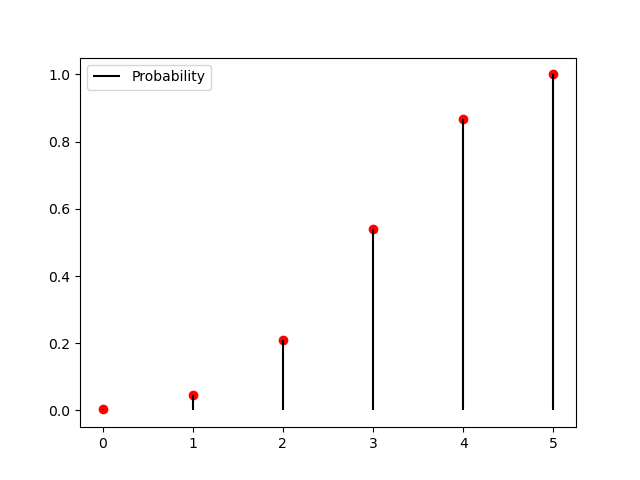
\includegraphics[width=\columnwidth]{CDF.png}
\caption{CDF}
\label{Fig1}
\end{figure}

\begin{figure}[h]
\centering
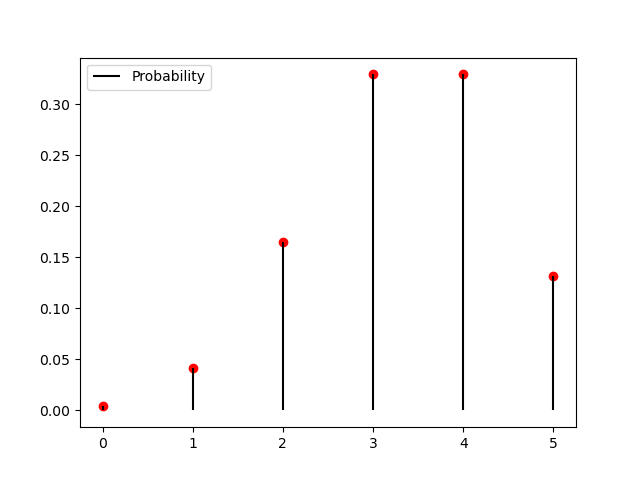
\includegraphics[width=\columnwidth]{PMF.png}
\caption{PMF}
\label{Fig2}
\end{figure}

\end{document}